%
% BUS 361: Project Management - A Course Overview
% Section: Planning
%
% Author: Jeffrey Leung
%

\section{Planning}
	\label{sec:planning}
\begin{easylist}

& To define a project:
	&& Create an idea and core message
	&& Create measures of performance
	&& Define resources and tasks
	&& Create budgets and schedule

& \textbf{Task definition:} Understanding of the quantification, assigning, tracking, completion, and evaluation of a task

& \textbf{Decomposition:} Breaking up a large project into manageable packages

\end{easylist}
\subsection{Work Breakdown Structure}
	\label{subsec:wbs}
\begin{easylist}

& \textbf{Work Breakdown Structure (WBS):} High-level breakdown of a project into cohesive, specific task descriptions
	&& Purposes are to:
		&&& Simplify complexity
		&&& Assign responsibility
		&&& Demonstrate progress
		&&& Assist in developing schedule and resource estimates
	&& Example: See figures~\ref{fig:wbs-example-diag} and \ref{fig:wbs-example-hier}

\begin{figure}[!htb]
	\caption{Work Breakdown Structure Example (Diagram)}
	\label{fig:wbs-example-diag}
	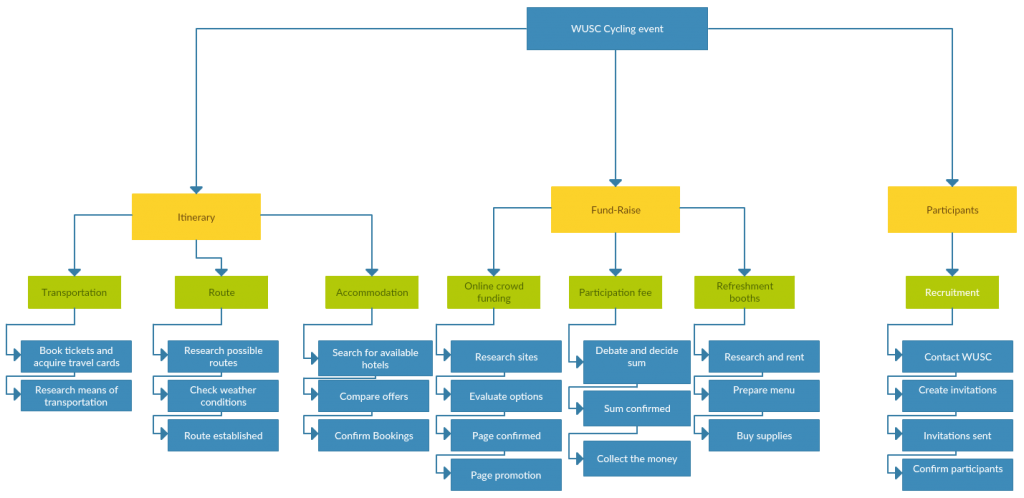
\includegraphics[width=\linewidth]{wbs-example-diag}
\end{figure}

\begin{figure}[!htb]
	\caption{Work Breakdown Structure Example (Hierarchy)}
	\label{fig:wbs-example-hier}
	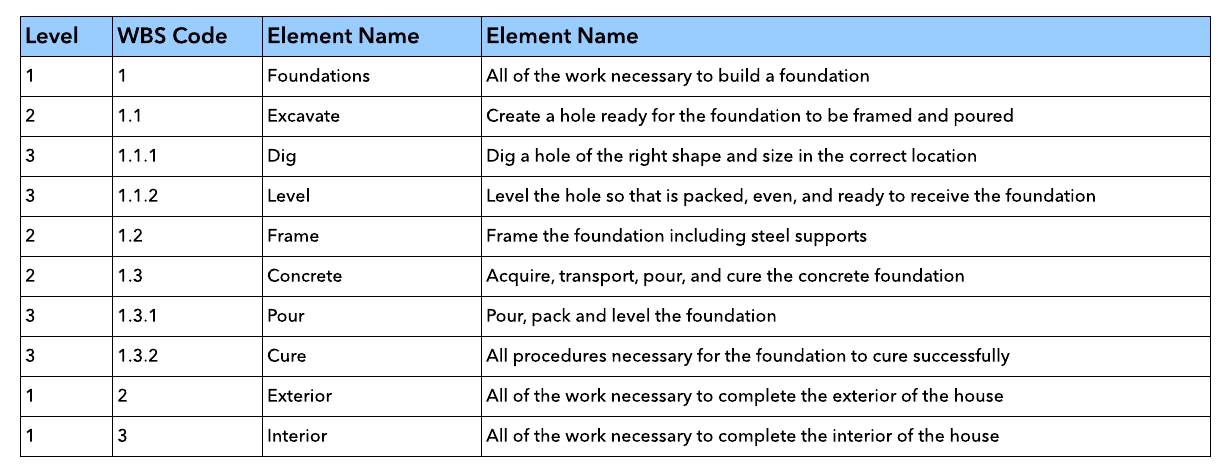
\includegraphics[width=\linewidth]{wbs-example-hier}
\end{figure}

	&& \textbf{Work package:} Unit of work which can be estimated, is a package which can be outsourced or contracted out, and produces a measurable deliverable
		&&& Smallest unit of a WBS
		&&& 8/80 hour rule: No work package should be less than 8 hours or more than 80 hours
		&&& Single reporting period rule: No set of work should be less than the reporting period (e.g. 2 weeks)
		&&& Should be sufficiently detailed to allow for cost and schedule estimates

\end{easylist}
\subsection{Network Diagram}
	\label{subsec:network-diagram}
\begin{easylist}

& \textbf{Network diagram:} Visual flow of the order in which work package are dependent on each other
	&& Conveys dependencies and chronological work order
	&& Conveys constraints such as:
		&&& Technical/causal constraint: Relationship between tasks where one task relies on the technical completion of the other
		&&& Management/discretionary constraint: Relationship between tasks where one task provides approval for the other to begin
		&&& Inter-project/resource constraint: Relationship between two tasks which are from separate areas (should be decoupled when possible to reduce risk)
		&&& Date constraint

\end{easylist}
\subsection{Estimations}
	\label{subsec:estimations}
\begin{easylist}

& \textbf{Top-down estimate:} Resource requirement estimate created from the requirements of top management
	&& Involves finish date, budget, resources, etc.
& \textbf{Bottom-up estimate:} Resource requirement estimate created from the analyses of the project manager and workers
& \textbf{Analogous estimate:} Resource requirement estimate created using a previous similar project
	&& \textbf{Parametric estimate:} Resource requirement estimate created using historical data with a multiplier for inflation, price increases, and other costs

& \textbf{Three Point Estimation:} Estimate generated from the weighted average of the most likely, pessimistic, and optimistic estimates

\end{easylist}
\begin{align*}
	TPE &= \frac{L + P + O}{3} \\
	\textrm{where } L &= \textrm{ most likely estimate} \\
	P &= \textrm{ pessimistic estimate} \\
	O &= \textrm{ optimistic estimate}
\end{align*}
\begin{easylist}

& Accuracy of estimates:
	&& \textbf{Ballpark estimate:} Estimate created with little time or information, and little accuracy (within 30\%)
	&& \textbf{Definitive estimate:} Estimate created with defined scope (within 5\%)

\end{easylist}
\clearpage
















